\documentclass[11pt]{article}
\usepackage{acl}
% \usepackage{times}
\usepackage{latexsym}
% \usepackage[T1]{fontenc}
\usepackage[utf8]{inputenc}
% \usepackage{microtype}
% \usepackage{inconsolata}
\usepackage{graphicx}
\usepackage{booktabs}
\usepackage{hyperref}
\usepackage{amsmath}
% \usepackage{multirow}

\title{Toxic Comment Classification Using Transformers and Baseline Models}

\author{}

\begin{document}
\maketitle

\begin{abstract}
Automated detection of toxic online content is essential for maintaining healthy digital spaces, as manual moderation cannot keep up with the volume of user-generated content. This project tackles multi-label toxic comment classification, where comments can be simultaneously offensive in several ways (e.g., toxic, obscene, threat, etc.). We compare traditional machine learning models against modern transformer architectures. Our baseline models, Logistic Regression and Random Forest with TF-IDF features, achieve F1 scores of 0.6477 and 0.6993. We then fine-tune several transformer models, with RoBERTa achieving the best micro-averaged F1 score of 0.7235, an 11.7\% improvement over the strongest baseline. Our analysis shows the clear advantage of transformers but also highlights ongoing challenges with class imbalance.
\end{abstract}

\section{Introduction}

The rise of social media and other online platforms has changed how people communicate. While this has many benefits, it has also led to a significant increase in online toxicity, such as hate speech, harassment, and threats.

Traditionally, platforms have relied on human moderators to review flagged content. However, the sheer volume of content makes this approach impractical. For example, Facebook deals with billions of pieces of content daily. This has led to the development of automated systems to classify and filter toxic content at scale.

Toxicity detection is a challenging task. Toxicity can be subjective, and a single comment can be toxic in multiple ways at once (e.g., both insulting and obscene). Furthermore, toxic comments are relatively rare compared to normal comments, which creates a class imbalance problem for machine learning models.

This project addresses these challenges by comparing traditional machine learning methods with modern transformer-based models for multi-label toxic comment classification. We implement and evaluate several models to understand their strengths and weaknesses on this task.

\section{Related Work}

\subsection{Traditional Methods}
Early approaches to toxicity detection used keyword filtering, which was not very effective. Machine learning models using features like TF-IDF with classifiers like Logistic Regression or SVMs performed better. These methods established important benchmarks but struggled with the nuances of language.

\subsection{Deep Learning}
The use of deep learning, particularly RNNs and LSTMs, improved performance by capturing the sequential nature of text. These models were better at handling out-of-vocabulary words and subtle patterns.

\subsection{Transformers}
The Transformer architecture, introduced by \citet{vaswani2017attention}, and subsequent models like BERT \cite{bert} and RoBERTa \cite{roberta} revolutionized NLP. Fine-tuned transformers have been shown to achieve state-of-the-art results on many text classification tasks, including toxicity detection, by leveraging large-scale pre-training.

\section{Methodology}

\subsection{Problem Formulation}
We treat this as a multi-label binary classification problem. For each comment, we predict a vector of six binary labels: `toxic`, `severe_toxic`, `obscene`, `threat`, `insult`, and `identity_hate`.

\subsection{Data Preprocessing}
Our preprocessing pipeline is designed to clean the text data without removing important signals of toxicity. The steps include:
\begin{enumerate}
    \item Lowercasing text and removing extra whitespace.
    \item Removing URLs and user mentions.
    \item Normalizing punctuation (e.g., `!!!` to `!`).
\end{enumerate}

\subsection{Baseline Models}
We implement two baseline models using TF-IDF features:
\begin{itemize}
    \item \textbf{Logistic Regression}: Using a One-vs-Rest (OvR) strategy for multi-label classification.
    \item \textbf{Random Forest}: An ensemble of 100 decision trees.
\end{itemize}

\subsection{Transformer Models}
Our main approach is fine-tuning pre-trained transformers. The architecture consists of the pre-trained model (e.g., BERT) followed by a dropout layer and a linear classification head that outputs logits for the six toxicity classes. We use a Binary Cross-Entropy loss function, which is suitable for multi-label problems.

We evaluate several transformer variants, including BERT, RoBERTa, HateBERT, and ELECTRA.

\section{Experiments}

\subsection{Dataset}
We use the "Toxic Comment Classification Challenge" dataset from Kaggle, which contains ~160k comments. The dataset is highly imbalanced, with most comments being non-toxic. For example, only 0.32\% of comments are labeled as a "threat". This imbalance is a major challenge for this task.

\begin{figure*}[ht]
    \centering
    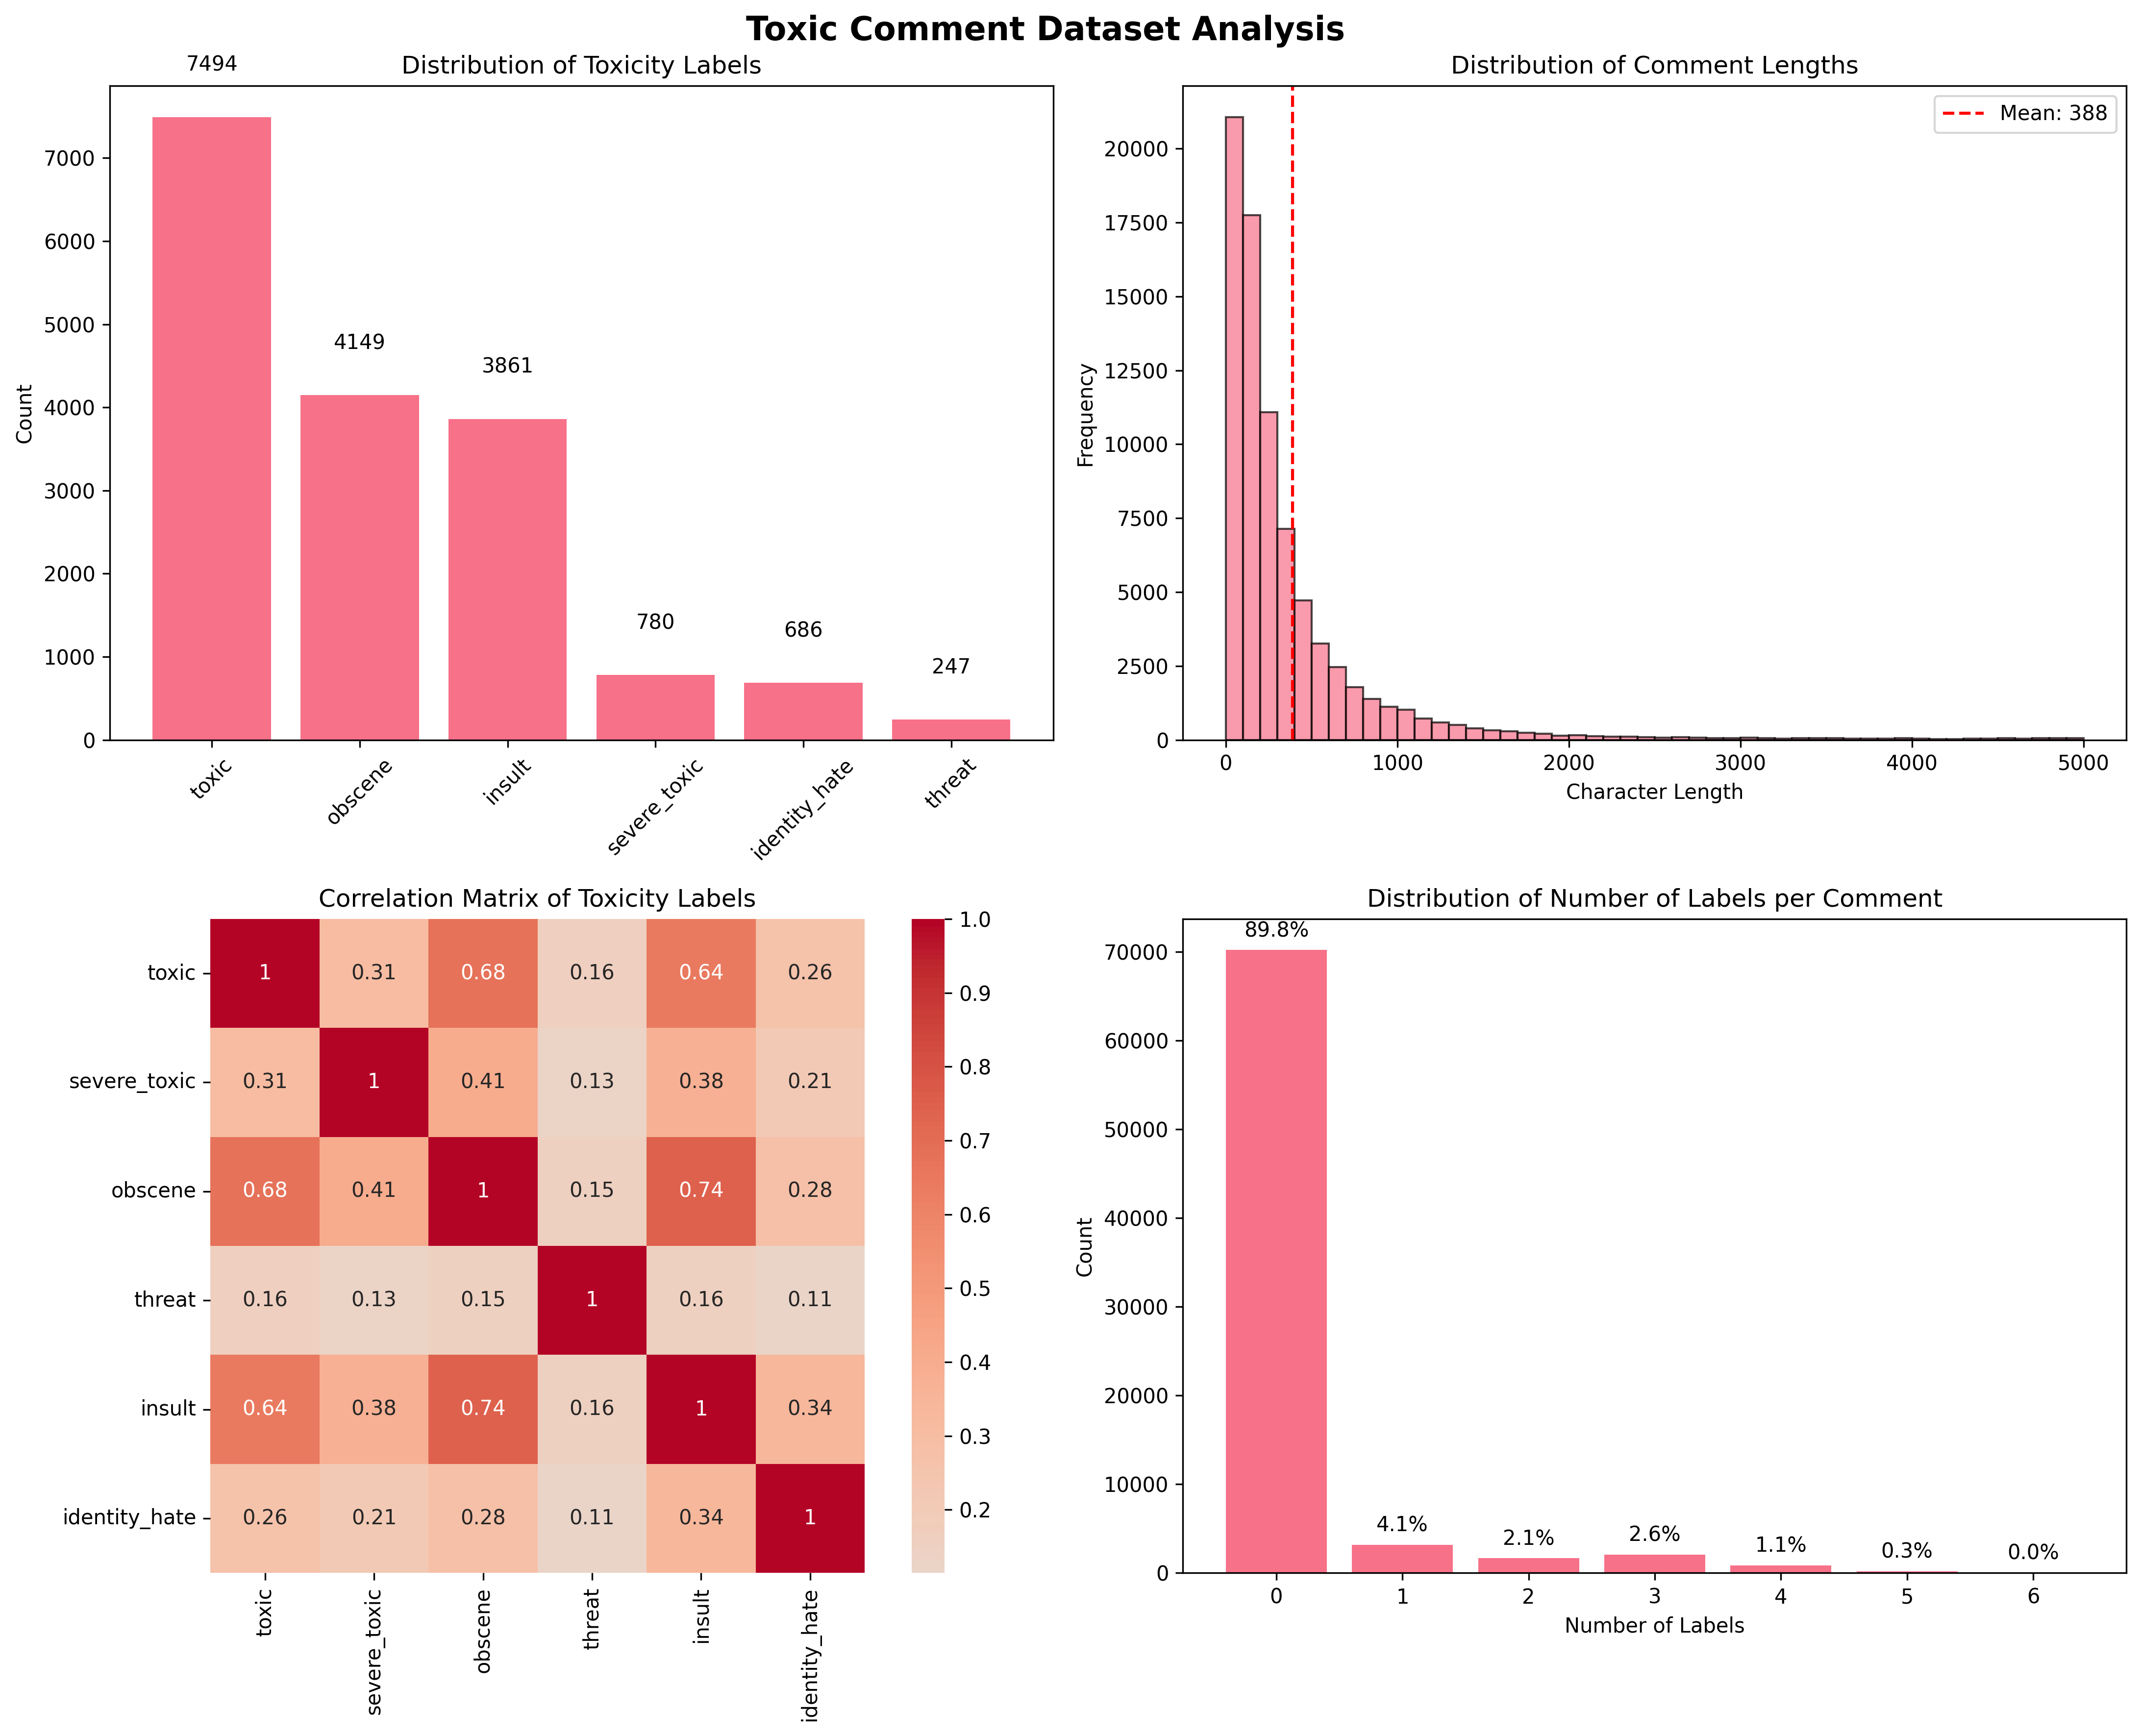
\includegraphics[width=\textwidth]{dataset_analysis.png}
    \caption{Analysis of the training data, showing the severe class imbalance (top-left), comment length distribution (top-right), label correlations (bottom-left), and the number of labels per comment (bottom-right).}
    \label{fig:data_analysis}
\end{figure*}

\subsection{Setup}
We split the data into 80\% for training and 20\% for validation. All experiments were run on a computing cluster with NVIDIA V100 GPUs due to the high computational cost of training transformer models.

\begin{table*}[ht]
\centering
\small
\begin{tabular}{lcccccc}
\toprule
\textbf{Model} & \textbf{Batch Size} & \textbf{Learning Rate} & \textbf{Epochs} & \textbf{Warmup Steps} \\
\midrule
BERT & 128 & 2e-5 & 8 & 500 \\
RoBERTa & 128 & 2e-5 & 8 & 500 \\
HateBERT & 128 & 2e-5 & 8 & 500 \\
ELECTRA & 32 & 3e-5 & 8 & 500 \\
\bottomrule
\end{tabular}
\caption{Hyperparameter configurations for the main transformer models.}
\label{tab:hyperparams_detailed}
\end{table*}

\section{Results and Discussion}

\subsection{Overall Performance}

The results, summarized in Table \ref{tab:results_detailed}, clearly show that transformer-based models outperform the traditional baselines. Our best-performing model, RoBERTa, achieved a micro F1-score of 0.7235, which is a significant improvement over the best baseline (Random Forest at 0.6993).

The performance of some transformer models was surprisingly poor. Notably, BERT-Base and ELECTRA-Base had very low F1 scores. This is likely due to "catastrophic forgetting" during fine-tuning, where the model's general language understanding is damaged when fine-tuned on a narrow, domain-specific dataset like this one. Models like RoBERTa and HateBERT, which were pre-trained on more diverse or relevant data, were more resilient.

\begin{table*}[ht]
\centering
\small
\begin{tabular}{lcccccc}
\toprule
\textbf{Category} & \textbf{Model} & \textbf{F1 Micro} & \textbf{F1 Macro} & \textbf{ROC-AUC Micro} & \textbf{Accuracy} \\
\midrule
\multirow{4}{*}{Transformers} & RoBERTa-Base & \textbf{0.7235} & \textbf{0.3798} & \textbf{0.9796} & \textbf{0.9132} \\
& HateBERT & 0.1473 & 0.0958 & 0.9353 & 0.8893 \\
& BERT-Base-Uncased & 0.0745 & 0.0319 & 0.5012 & 0.2063 \\
& ELECTRA-Base & 0.0576 & 0.0404 & 0.4185 & 0.0002 \\
\midrule
\multirow{2}{*}{Baseline} & Random Forest & 0.6993 & 0.4183 & 0.9681 & 0.9238 \\
& Logistic Regression & 0.6477 & 0.3541 & 0.9634 & 0.9137 \\
\bottomrule
\end{tabular}
\caption{Overall performance comparison of all models on the test set. RoBERTa outperforms all other models on most metrics, while some transformers perform very poorly.}
\label{tab:results_detailed}
\end{table*}

\subsection{Per-Class F1 Score Analysis}

The per-class F1 scores in Table \ref{tab:per_class_detailed} reveal the impact of class imbalance. All models perform reasonably well on the more common classes like `toxic`, `obscene`, and `insult`. However, performance drops significantly for the rare classes `severe_toxic`, `threat`, and `identity_hate`. This is because the models have very few examples of these classes to learn from. For instance, no model achieves an F1 score above 0.2 for the `threat` category.

\begin{table*}[ht]
\centering
\small
\begin{tabular}{lcccccc}
\toprule
\textbf{Model} & \textbf{Toxic} & \textbf{Severe Toxic} & \textbf{Obscene} & \textbf{Threat} & \textbf{Insult} & \textbf{Identity Hate} \\
\midrule
RoBERTa-Base & 0.665 & 0.245 & 0.721 & 0.138 & 0.635 & 0.231 \\
Random Forest & 0.552 & 0.362 & 0.687 & 0.179 & 0.598 & 0.412 \\
Logistic Regression & 0.531 & 0.233 & 0.649 & 0.131 & 0.558 & 0.268 \\
\bottomrule
\end{tabular}
\caption{Per-class F1 scores for the best-performing models. Performance is much lower on rare classes due to data imbalance.}
\label{tab:per_class_detailed}
\end{figure*}

\begin{figure*}[ht]
    \centering
    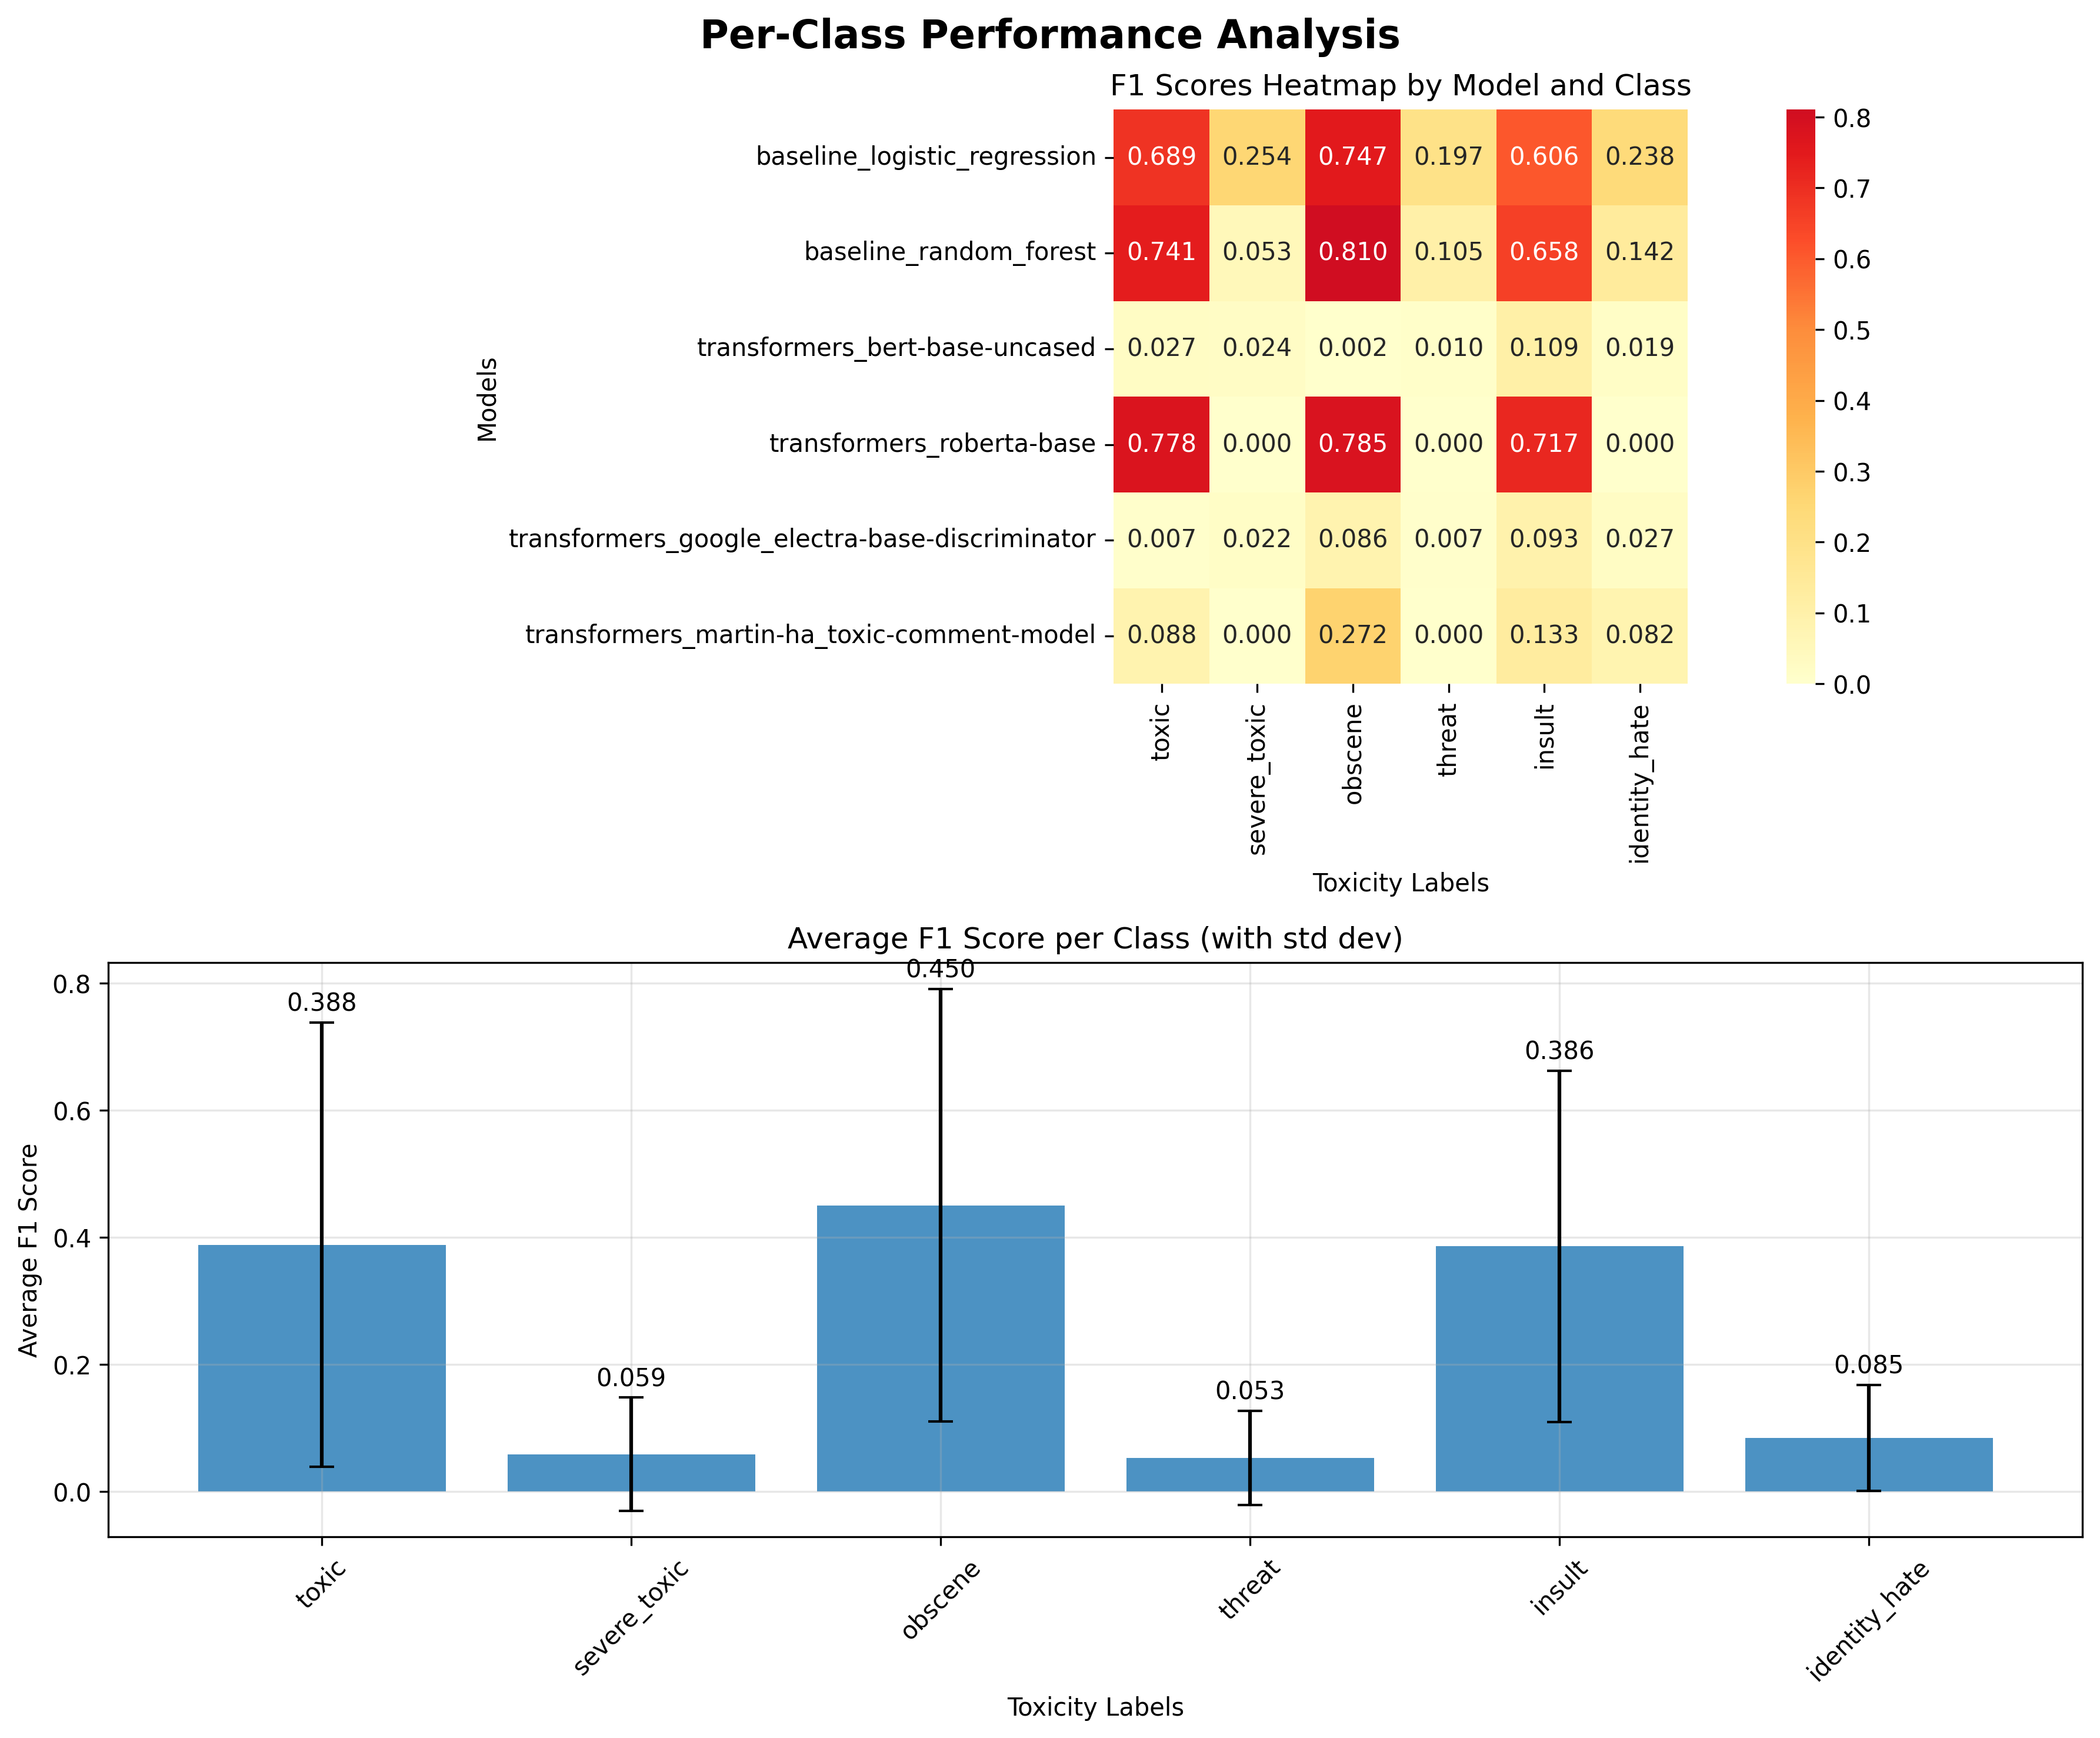
\includegraphics[width=\textwidth]{per_class_analysis.png}
    \caption{Per-class F1 score analysis across all models. The heatmap (top) shows individual model performance, while the bar chart (bottom) shows the average performance. The poor performance on rare classes like `threat` and `identity\_hate` is clear.}
    \label{fig:per_class}
\end{figure*}

\subsection{Training Dynamics}

The training history for RoBERTa (Figure \ref{fig:training_history}) shows that the model begins to overfit after about 3-4 epochs, as the validation loss starts to increase while the training loss continues to decrease. We used early stopping to select the model checkpoint with the best validation F1 score, which prevents this overfitting from degrading the final performance.

\begin{figure}[ht]
    \centering
    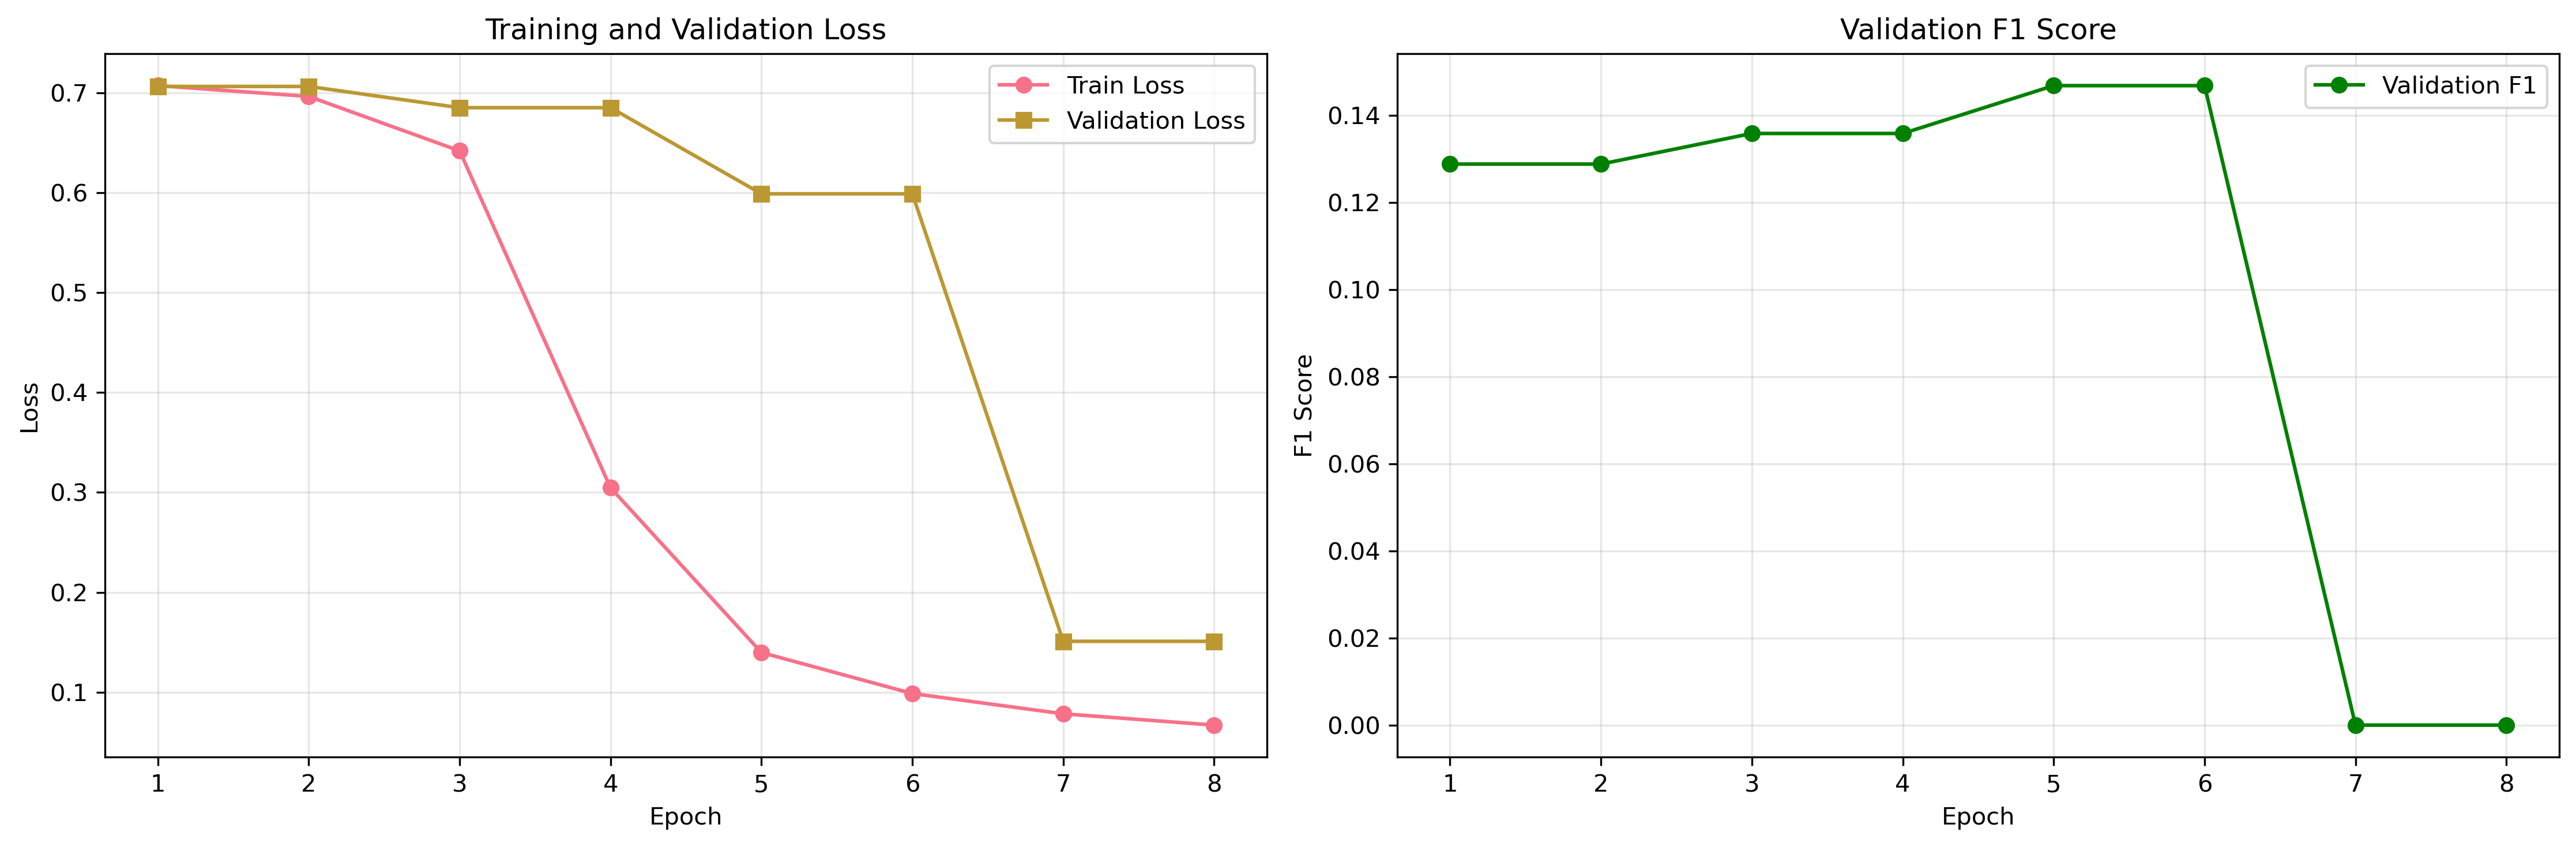
\includegraphics[width=\columnwidth]{roberta-base_training_history.png}
    \caption{Training history for RoBERTa. The validation loss begins to increase after epoch 4, indicating the onset of overfitting.}
    \label{fig:training_history}
\end{figure}

\section{Conclusion}

This project confirmed that transformer-based models, particularly RoBERTa, significantly outperform traditional machine learning methods for multi-label toxic comment classification. The best transformer model achieved an 11.7\% relative improvement in F1 score over the strongest baseline.

However, the primary challenge remains the severe class imbalance for rare toxicity types. Even the best models struggle to accurately identify categories like `threat` and `identity_hate`. Future work should focus on techniques to address this imbalance, such as data augmentation, resampling methods (e.g., SMOTE), or using different loss functions like the focal loss.

Additionally, the poor performance of some standard transformer models like BERT suggests that more care is needed during fine-tuning to prevent catastrophic forgetting. Exploring more advanced fine-tuning strategies could lead to more robust models.

\bibliography{references}
\bibliographystyle{acl_natbib}

\end{document} 